\section{Akcelerometr trzyosiowy}
W latach 90 akcelerometry instalowano jedynie w roli mechanizmów służących do
uruchamiania poduszek powietrznych w samochodzie w przypadku wystąpienia
zderzenia. W chwili obecnej akcelerometry wykonane w technologii
MEMS\footnote{MEMS - } 
można znaleźć w większości urządzeń codziennego użytku tj.
telefony komórkowe, konsole do gier, komputery przenośne czy cyfrowe aparaty
fotograficzne. Powodem tak spektakularnego wzrostu popularności było pełne
rozwinięcie się technologii MEMS. W dobie miniaturyzacji fakt, iż w miejsce do
niedawna używanych urządzeń można wstawić pojedynczy układ
scalony jest jednym z podstawowych powodów dla których, między innymi,
akcelerometry cieszą się tak szerokim spektrum zastosowań. Jednakże, ceną tak
daleko idącej miniaturyzacji jest spadek duży dokładności pomiarowej w
porównaniu do akcelerometrów opartych o tensometry. Jak się jednak okazuje, do
codziennego użytku precyzja oferowana przez tego typu czujniki jest w zupełności wystarczająca.

Bardzo dobrym przykładem zastosowania akcelerometru jest dostępna w większości
aparatów cyfrowych funkcja optycznej stabilizacji obrazu (Optical Image
Stabilization). Funkcja ta polega na redukcji zniekształceń  spowodowanych
drżeniem rąk fotografa w~trakcie akwizycji obrazu. Problem jest tym poważniejszy
iż nieustanna miniaturyzacja urządzeń dodatkowo wzmacnia mimowolne\footnote{Ręka
przeciętnego człowieka drży mimowolnie z częstotliwością od 10 do 20 Hz} drżenie
rąk użytkownika. Dlatego też większość aparatów wyposażonych jest czujniki które
mierzą wspomniane drgania, a następnie uzyskane informacje przekazują do modułu
sterującego położeniem soczewek i przetwornika obrazu. Następnie moduł ten
dostosowuje parametry pracy aparatu tak aby zminimalizować wpływ nieporządanych przeunięć
na efekt końcowy pracy jakim jest zdjęcie.

Innym popularnym przykładem zastosowania akcelerometrów są pedometry, potocznie 
nazywane krokomierzami. Dzięki zastosowanej technologii czujniki w krokomierzach
mogą dokonywać równocześnie pomiaru względem trzech osi. Co więcej tego typu
urządzenia umożliwiają dokonywanie pomiarów niemal całkowicie niezależne od
swojej orientacji, a ich niewielkie rozmiary pozwalają na ich integrację z 
dowolnymi urządzeniami mobilnymi. Akcelerometry wykonane w technologi MEMS
najlepiej sprawdzają się  podczas pomiaru przyspieszenia statycznego
pozwalającego jednoznacznie wyznaczyć kąt odchylenia urządzenia względem pionu. 
Można nimi dokonywać również pomiaru przyspieszenia dynamicznego pojawiającego 
się na skutek wibracji, uderzenia czy innego rodzaju ruchu. Pomimo swoich
licznych zalet akcelerometry MEMS posiadają pewne ogrniczenia które mogą być
bardzo istotne podczas projektowania bardziej skomplikowanych systemów
czujników. Jedynym z podstawowych problemów jest brak możliwości uzyskania
jednoznacznej informacji na temat orientacji urządzenia zarówno w pionie jak i
poziomie. W ramach przykładu spróbujmy przeanalizować wykorzystanie
akcelerometru do przełączania widoku na ekranie w zależności od jego orientacji.  W przypadku
gdy oś X lub Y są równoległe z wektorem grawitacji na podstawie informacji z
akcelerometru można w bardzo prosty sposób ustalić w jakim położeniu znaduje
się aktualnie urządzenie. 

\begin{figure}[h!]
 \centering
 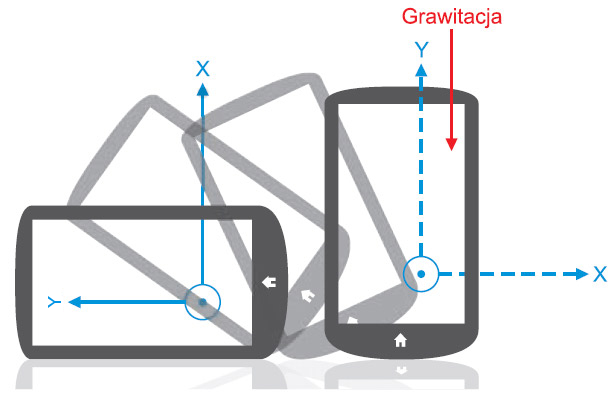
\includegraphics[height=62mm]{../images/ch04/acc_orientation.png}
 \caption{}
 \label{fig:AkcelerometrOrientation}
\end{figure}
%TODO
Jednak w momencie, gdy osie wyświetlacza są prostopadłe do wektora grawitacji
(rys. 5), informacja z akcelerometru w tym zakresie nie jest użyteczna. Ponadto
tam, gdzie akcelerometr jest używany jako czujnik odchylenia od pionu, konieczne
jest wyizolowanie sygnału będącego skutkiem wyłącznie wpływu grawitacji, który
posłuży dalej jako odniesienie. Sygnał taki można jednak wyodrębnić jedynie
wówczas, gdy akcelerometr jest nieruchomy, co w przypadku interfejsów użytkownika
wymagających informacji o odchyleniu może destabilizować pracę.

Innym sposobem na wyodrębnienie informacji o odchyleniu od pionu jest
wykorzystanie filtru dolnoprzepustowego. Przyjmuje się wówczas założenie, że
sygnał odpowiadający przyspieszeniu dynamicznemu ma dużą częstotliwość i można go
odfiltrować. Jednocześnie należy też założyć, że ruchy odchylające obiekt od
pionu są wolne, w związku z czym szybsze zmiany orientacji obiektu także zostaną
odfiltrowane, a wówczas informacja o kącie nachylenia będzie niedokładna. By
pokonać opisywane ograniczenia, najczęściej dane z akcelerometrów przetwarza się
w połączeniu z informacją z innych czujników, np. z żyroskopu.

\subsection{Rodzaje akcelerometrów}
Istnieje wiele różnych rodzaji akcelerometrów. Akcelerometry mechaniczne
przypominają po części zachowanie pasażera w samochodzie który gwałtowanie
przyspiesza i zwalnia. Posiadają one element masy przyczepiony do elementu
sprężynowego umieszczonego w całości w zewnętrznej obudowie. Kiedy taki
akcelerometr zacznie przyspieszać obudowa zewnętrzna przemieści się podczas gdy
punkt masy wychyli się w kierunku przeciwnym do przyspieszenia co spowoduje
rozciągnięcie się sprężyny wprostproporcjonalne do siły która spowodowała
przyspieszenie. Mierząc więc odległość na jaką nastąpiło wychylenie jesteśmy w
stanie wartość działającej siły jak również wartość przyspieszenia. Opisana
powyżej zasada pomiaru leży u podstaw działania sesjsmografów które za pomocą
masy dołączonej do elementu piśmiennego rejestrują siły występujące w chwili
trzęsienia ziemi. 

Alternatywnym podejściem jest wykorzystanie sygnałów elektrycznych i
magnetycznych do pomiaru przyspieszenia. Wśród tego rodzaju akcelerometrów
możemy wyróżnić następujące trzy najpopularniesze typy: akcelerometr
piezorezystywny, akcelerometr pojemnościowy, akcelerometr piezoelektryczny.
Istnieją również akcelerometry które dokonują pomiaru przyspieszenia w oparciu o
efekt Halla. 

\begin{figure}[h!]
 \centering
 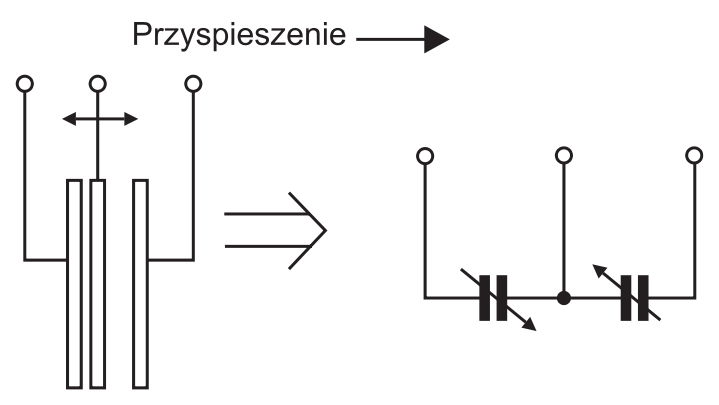
\includegraphics[height=62mm]{../images/ch04/acc_intro.png}
 \caption{Schemat ideowy akcelerometu dokonującego pomiaru wzdłuż jednej osi}
 \label{fig:AkcelerometrIdeowyScheamt}
\end{figure}

Przyspieszomierze piezorezystywne mają punkt masy dołączony do
potencjometru który zachowuje się jak regulator głośności który zwiększa i
zmniejsza przepływ prądu w zależności od siły jaka oddziaływuje na czujnik.
Bardzo podobą zasadę działania wykazują akcelerometry pojemnościowe te jednak
wykorzystują efekt zmiany pojemności kondensatorów zastosowanych w miejscu w
którym poprzednio użyto potnecjometru. Ostatnim rodzajem akcelerometrów są
urządzeniami bazujące na piezoelektrycznych kryształach takich jak na przykład
kwarc. Punkt masy naciska na kryształ pod wpływem przyspieszenia co powoduje, że
powstawanie napięcia które jest wykorzystywane do wykonywania pomiaru. 


\subsubsection{Algorytm rozpoznawania kroków}
Do poprawnego działania algorytmu wymagane jest wykorzystanie akcelerometru
trójosiowego. Dzięki zastosowaniu urządzenia tego typu jesteśmy w stanie
wyeliminować problemy wynikające z konieczności uwzględnienia aktualnego
wychylenia akcelerometru względem kierunku siły przyciągania.
